\documentclass{article}
\usepackage{german}
\usepackage[latin1]{inputenc}
\usepackage{a4wide}
\usepackage{amssymb}
\usepackage{fancyvrb}
\usepackage{alltt}
\usepackage{epsfig}
\usepackage{hyperref}
\usepackage{fancyhdr}
\usepackage{lastpage} 
\usepackage{color}
\hypersetup{
	colorlinks = true, % comment this to make xdvi work
	linkcolor  = blue,
	citecolor  = red,
        filecolor  = blue,
        urlcolor   = [rgb]{0.5, 0.4, 0.0},
	pdfborder  = {0 0 0} 
}

\pagestyle{fancy}

\fancyfoot[C]{--- \thepage/\pageref{LastPage}\ ---}

\renewcommand{\labelenumi}{(\alph{enumi})}
\renewcommand{\labelenumii}{\arabic{enumii}.}

\begin{document}
\noindent
{\Large \textbf{Aufgaben-Blatt}: Das $3 \times 3$-Schiebe-Puzzle}
\vspace{0.5cm}


Ein $3 \times 3$-Schiebe-Puzzle wird auf einem quadratischen Spielfeld der Seitenl�nge 3 gespielt.
Dieses Spielfeld ist in $3 \times 3 = 9$ quadratische Felder unterteilt.   Auf 8 der Felder liegen 
quadratischen Kacheln der Seitenl�nge 1, w�hrend ein Feld frei bleibt.  Die 8 Kacheln
sind mit den Zahlen von 1 bis 8 durchnummeriert.  Abbildung \ref{fig:8-puzzle.eps} zeigt zwei
verschiedene Stellungen des Schiebe-Puzzles.  

\begin{figure}[!ht]
\centering
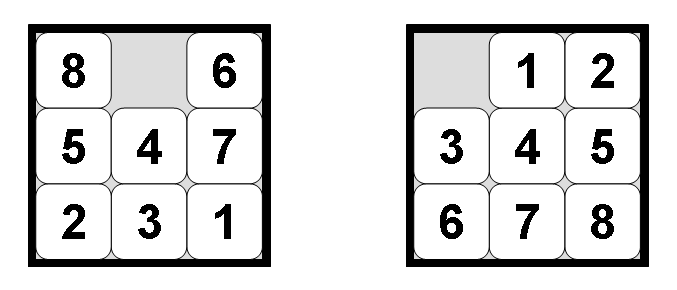
\epsfig{file=8-puzzle, scale=0.6}  
\caption{Das $3 \times 3$-Schiebe-Puzzle.}
\label{fig:8-puzzle.eps}
\end{figure}

Die Aufgabe bei diesem Schiebe-Puzzle besteht darin, die auf der linken Seite der Abbildung gezeigte
Konfiguration in die auf der rechten Seite der Abbildung gezeigte Konfiguration zu �berf�hren.
Dabei sind die folgenden Operationen erlaubt:
\begin{enumerate}
\item Falls eine Kachel links neben dem freien Feld liegt, kann diese nach rechts auf das freie Feld
      geschoben werden.  
\item Falls eine Kachel rechts neben dem freien Feld liegt, kann diese nach links auf das freie Feld
      geschoben werden.  
\item Falls eine Kachel unter dem freien Feld liegt, kann diese nach oben auf das freie Feld
      geschoben werden.  
\item Falls eine Kachel �ber dem freien Feld liegt, kann diese nach unten auf das freie Feld
      geschoben werden.  
\end{enumerate}
Um einen Eindruck davon zu bekommen, wie sich dieses Puzzle l�sen l�sst, k�nnen Sie es auf der Seite
\\[0.2cm]
\hspace*{1.3cm}
\href{http://mypuzzle.org/sliding}{http://mypuzzle.org/sliding}
\\[0.2cm]
ausprobieren.  Ziel dieser Aufgabe ist die Entwicklung eines  \textsc{SetlX}-Programms, das eine
L�sung des oben gezeigte Puzzles berechnen kann.  
Laden Sie dazu von meiner Seite das Programm
\\[0.2cm]
\hspace*{-0.8cm}
\href{https://github.com/karlstroetmann/Logik/blob/master/Aufgaben/Blatt-6/sliding-frame.stlx}{\texttt{https://github.com/karlstroetmann/Logik/blob/master/Aufgaben/Blatt-6/sliding-frame.stlx}} 
\\[0.2cm]
herunter.  Bei meinem Programm gehe ich davon aus, dass ein Zustand des Schiebe-Puzzles als eine
Liste dargestellt wird, die 3 Listen der L�nge 3 enth�lt.  Jede dieser Listen stellt dabei eine
Zeile des Schiebe-Puzzles dar.  Das leere Feld wird dabei durch die Zahl $0$ dargestellt.  Die in
der obigen Abbildung angegebenen Instanzen des Puzzles lassen sich daher durch die beiden Listen
\pagebreak

\begin{verbatim}
    start := [ [8, 0, 6],
               [5, 4, 7],
               [2, 3, 1] 
            ];
\end{verbatim}
beziehungsweise
\begin{verbatim}
    goal  := [ [0, 1, 2],
               [3, 4, 5],
               [6, 7, 8] 
             ];
\end{verbatim}
darstellen.  Sie k�nnen sich �berlegen, dass es insgesamt $9! = 1 \cdot 2 \cdot 3 \cdot \mbox{\dots} \cdot 8 \cdot 9$
verschiedene Konfigurationen des Schiebe-Puzzles gibt.  Da diese Zahl bereits recht gro� ist,
verbietet es sich, die Relation, welche die verschiedenen Zustands�berg�nge beschreibt, explizit als
Menge darzustellen.  Stattdessen k�nnen Sie diese Relation durch eine Funktion 
\\[0.2cm]
\hspace*{1.3cm}
$\texttt{nextStates}(s)$
\\[0.2cm]
darstellen, die f�r eine gegebene Konfiguration $s$ des Schiebe-Puzzles die Menge aller der
Konfigurationen berechnet, die in einem Schritt berechnet werden k�nnen.  Die Funktion
\texttt{findPath}, die in Zeile 30 der Datei \texttt{sliding-frame.stlx} definiert wird, wird nun 
in der Form 
\\[0.2cm]
\hspace*{1.3cm}
$\texttt{findPath}(\textsl{start}, \textsl{goal}, \textsl{nextStates})$
\\[0.2cm]
aufgerufen.  Hier ist \textsl{start} die Ausgangs-Konfiguration, \textsl{goal} ist die
Ziel-Konfiguration und \textsl{nextStates} ist die Funktion, die f�r eine gegebene Konfiguration die
Menge aller Konfigurationen berechnet, die in einem Schritt von dieser Konfiguration
erreicht werden k�nnen.  Ihre Aufgabe beschr�nkt sich darauf, die Definition der Funktion
\texttt{nextStates} in Zeile 56 zu vervollst�ndigen.  Es ist sinnvoll, wenn Sie sich geeignete
Hilfs-Prozeduren �berlegen, mit deren Hilfe Sie diese Aufgabe l�sen k�nnen.  Sobald Sie die Prozedur
\texttt{nextStates} korrekt implementiert haben, berechnet das Programm eine m�gliche L�sung.
\vspace*{0.3cm}

\noindent
\textbf{Hinweis}:  Auf meinem Rechner\footnote{
  Dabei handelt es sich um eine iMac mit einem 2,7 GHz Intel Core i5 aus dem Jahr 2011.
} 
ben�tigt das Programm knapp 22 Sekunden und belegt in der Spitze etwas mehr als 1 Gigabyte Speicher.
Bei der  berechneten L�sung wird  31 mal eine Kachel verschoben.  Bei der Berechnung der L�sung
werden insgesamt $181440 = 9!/2$ verschieden Konfigurationen untersucht. 
\end{document}

%%% Local Variables: 
%%% mode: latex
%%% TeX-master: t
%%% End: 
